% 隔離テスト用ドライバ: スライド11 のみを単独ビルド（共有 main.tex には触れない）
% ページ番号を 11 に偽装し帯色 barC・本文 HeaderBlue 連動を本番一致させる。
\documentclass[11pt,aspectratio=43,dvipsnames]{beamer}
\usepackage{luatexja}
\usepackage[match]{luatexja-fontspec}
\setmainjfont{HaranoAjiGothic}
\setsansjfont{HaranoAjiGothic}
\renewcommand{\kanjifamilydefault}{\gtdefault}
\usepackage{amsmath, amssymb}
\usepackage[version=4]{mhchem}
\usepackage{booktabs}
\usepackage{multirow}
\usepackage{colortbl}
\usepackage{graphicx}
\graphicspath{{figures/}}
\usepackage{pgfplots}
\pgfplotsset{compat=1.18}
% =====================================================================
%  seminar テーマ定義（既存 Marp デザインの Beamer 再現）
%  ・濃青の恒常ヘッダーバー（セクション名＋ページ番号）
%  ・専用表紙（アクセントライン＋グラデ背景）
%  ・本文は白地・濃青見出し
%  main.tex から \input する（パッケージではなく生プリアンブル）
% =====================================================================

% ---- ベース：装飾の少ないテーマから組む -----------------------------
\usetheme{default}
\usefonttheme{professionalfonts}
\setbeamertemplate{navigation symbols}{}   % ナビゲーション記号を消す

% ---- TikZ（ヘッダー・表紙・矢印などで使用）-------------------------
\usepackage{tikz}
\usetikzlibrary{arrows.meta, positioning, calc, shapes.geometric, fit, patterns}

% ---- 配色（ルール準拠）---------------------------------------------
\definecolor{HeaderBlue}{HTML}{0f5a7a}   % ヘッダー・見出しの濃青
\definecolor{DateGray}{HTML}{334b5e}     % 表紙の日付グレー
\definecolor{TitleBG}{HTML}{edf5fb}      % 表紙グラデの薄青

% コンテンツ用パレット（図・ハイライト・矢印で共通利用）
\definecolor{ArrowBlue}{HTML}{1F6FC4}    % 矢印・強調の青
\definecolor{HiPink}{HTML}{F4B6BE}       % ハイライト見出し（暖色）
\definecolor{HiBlue}{HTML}{C7DCEF}       % ハイライト見出し（寒色）
\definecolor{IpaBlue}{HTML}{1F5FC4}      % グラフ系列1（青）
\definecolor{DipeOrange}{HTML}{E8821E}   % グラフ系列2（橙）
\definecolor{SpRed}{HTML}{C0392B}        % 反応式：プロピレン強調の赤
\definecolor{SpBlue}{HTML}{1F6FC4}       % 反応式：エテン・エタン・CH0.5 の青

% 帯（ヘッダーバー）のパート別配色（寒色グラデ）。本文枠線は HeaderBlue のまま。
%  1-4 導入・全体像／5-9 反応・反応器／10-13 分離／14-17 最適化・経済・結言
\definecolor{barA}{HTML}{0F5A7A}   % 1-4  青緑
\definecolor{barB}{HTML}{1D6E6E}   % 5-9  シアン寄り
\definecolor{barC}{HTML}{2E4C8A}   % 10-13 青
\definecolor{barD}{HTML}{4A3C84}   % 14-17 紫

\setbeamercolor{normal text}{fg=black, bg=white}
\setbeamercolor{frametitle}{fg=HeaderBlue, bg=white}
\setbeamercolor{itemize item}{fg=HeaderBlue}
\setbeamercolor{itemize subitem}{fg=HeaderBlue}
\setbeamercolor{block title}{fg=white, bg=HeaderBlue}
\setbeamercolor{block body}{fg=black, bg=TitleBG}
\setbeamercolor{alerted text}{fg=HeaderBlue}

% ---- フォントサイズ（Marp px をおおよそ pt に対応）------------------
\setbeamerfont{frametitle}{size=\large, series=\bfseries}   % スライド見出し ~44px

% ---- 恒常ヘッダーバー（headline）-----------------------------------
%  左：セクション名（無ければロゴ枠）／右：ページ番号
\newcommand{\HeaderLogo}{}   % ロゴを入れるなら \renewcommand で画像指定
% 本線の総枚数（分母）。appendix に入ると分子がこれを超え、本線/付録を見分けられる。
\newcommand{\MainTotal}{17}
% パート別に帯色を選ぶ：1-4=barA／5-9=barB／10-13=barC／14-17=barD。
% スライド4の独自帯（CC・GCC）など headline を上書きする箇所でも呼べるよう独立コマンド化。
% 併せて本文アクセント色 HeaderBlue 自体をそのパート色へ再定義し、各スライドの
% 図・枠線・矢印・ボックス（HeaderBlue 参照）をパート色に連動させる（\colorlet は大域的）。
% headline はフレーム本文より前に組まれるため、ここでの再定義が本文に効く。
\newcommand{\SetBarColor}{%
  \ifnum\insertframenumber<5\setbeamercolor{headerbar}{fg=white, bg=barA}\colorlet{HeaderBlue}{barA}%
  \else\ifnum\insertframenumber<10\setbeamercolor{headerbar}{fg=white, bg=barB}\colorlet{HeaderBlue}{barB}%
  \else\ifnum\insertframenumber<14\setbeamercolor{headerbar}{fg=white, bg=barC}\colorlet{HeaderBlue}{barC}%
  \else\setbeamercolor{headerbar}{fg=white, bg=barD}\colorlet{HeaderBlue}{barD}%
  \fi\fi\fi}
\setbeamertemplate{headline}{%
  \ifnum\insertframenumber>0\relax
    \SetBarColor
    \begin{beamercolorbox}[wd=\paperwidth, ht=4.5ex, dp=1.8ex,
                           leftskip=1.2em, rightskip=1.2em]{headerbar}%
      \color{white}\bfseries\large
      \insertsectionhead%
      \hfill
      \insertframenumber/\MainTotal%
    \end{beamercolorbox}%
  \fi
}
\setbeamercolor{headerbar}{fg=white, bg=barA}
\setbeamertemplate{footline}{}             % フッターは使わない
\setbeamersize{text margin left=3mm, text margin right=3mm}  % 本文を横幅ぎりぎりまで

% 【必須ルール】帯と本文の間の余白を詰める（全スライド共通）。
%  beamer 既定の天井スキップで本文が帯から離れるのを、headline 直後の負スキップで打ち消す。
%  情報量最優先：無駄な上余白は作らない。各スライドは [t] 推奨。
\addtobeamertemplate{headline}{}{\vskip-2.6ex}

% frametitle はバーの直下に置く（左寄せ・濃青・太字）
\setbeamertemplate{frametitle}{%
  \vskip0.6ex
  \hspace{0.6em}\usebeamerfont{frametitle}\usebeamercolor[fg]{frametitle}\insertframetitle\par
  \vskip0.2ex
}

% ---- 箇条書きをシンプルに ------------------------------------------
\setbeamertemplate{itemize item}{\textbullet}
\setbeamertemplate{itemize subitem}{--}

% =====================================================================
%  再利用ヘルパー（どのスライドでも使える共通部品）
% =====================================================================
% 青い矢印 →（行中に置ける。結論や対応関係の明示に）
\newcommand{\bluearrow}{\tikz[baseline=-0.5ex]\draw[ArrowBlue, line width=1pt,
  -{Stealth[length=2.2mm]}] (0,0)--(0.55,0);}

% ハイライト見出し  \hilite{色}{テキスト}  例: \hilite{HiPink}{IPA選択率の温度依存性}
\newcommand{\hilite}[2]{\colorbox{#1}{\bfseries\normalsize #2}}

% パラメータ表  \paramtable{ 項目 & 値 \\ ... }  （左:項目 右:値、単位は数式推奨）
\newcommand{\paramtable}[1]{%
  {\footnotesize\renewcommand{\arraystretch}{1.15}%
   \begin{tabular}{@{\hspace{1em}}ll@{}}#1\end{tabular}}}

% =====================================================================
%  専用表紙コマンド  \seminartitlepage
%  ルール準拠：アクセントライン(120x8px相当) + 160度グラデ背景
%               h1 60px / h2 34px濃青 / 著者27px / 日付22pxグレー
%  使い方: \title{} \subtitle{} \author{} \date{} を設定後に呼ぶ
% =====================================================================
\newcommand{\seminartitlepage}{%
  \begin{frame}[plain]
    \begin{tikzpicture}[remember picture, overlay]
      % 背景グラデ（左上 薄青 → 右下 白、斜め）
      \shade[top color=TitleBG, bottom color=white, shading angle=20]
        (current page.south west) rectangle (current page.north east);
      % アクセントライン（上から少し下げて左に）
      \fill[HeaderBlue]
        ([xshift=9mm, yshift=-12mm]current page.north west)
        rectangle ++(16mm, 1.1mm);
      % テキストブロック（左寄せ・縦中央付近）
      \node[anchor=center, text width=0.86\paperwidth, align=center]
            at (current page.center) {%
        {\fontsize{22pt}{28pt}\selectfont\bfseries\color{black}\inserttitle\par}
        \vspace{0.3em}
        {\fontsize{16pt}{20pt}\selectfont\bfseries\color{HeaderBlue}\insertsubtitle\par}
        \vspace{1.0em}
        {\fontsize{13pt}{17pt}\selectfont\color{black}\insertauthor\par}
        \vspace{0.4em}
        {\fontsize{11pt}{14pt}\selectfont\color{DateGray}\insertdate\par}
      };
    \end{tikzpicture}
  \end{frame}
}

\begin{document}
\setcounter{framenumber}{10}   % 次フレームが 11 になる（帯 barC・11/17 表示）
\section{蒸留分離}
% =====================================================================
%  11  蒸留塔設計 — 左上=諸元表／右上=実寸比タワー図／下は空ける
%  source_memo: 05/06/07章＋trial #201。脱ブタン C3H8/C4H10 36段33m P19.5 全凝縮 α大／
%   脱エタン C2H6/C3H8 61段52m P7.9 部分凝縮 α3.9／C3 C3H6/C3H8 117段94m P16.7 全凝縮 α1.07(最難)。
%  方針：タイトル・共通設計枠組み・モデル名(SM/HYSYS)は載せない。表(左上)＋実寸比タワー(右上)。
%   下半分は意図的に空ける(後で別要素)。色は最難C3の赤のみ。丸括弧禁止。
% =====================================================================
\begin{frame}[t]

  \vspace{-0.7em}

  \begin{columns}[T,onlytextwidth]
    % ===== 左上：諸元表（SM/HYSYS は載せない／塔高は図側）=========
    \begin{column}{0.64\textwidth}
      {\scriptsize
       \setlength{\tabcolsep}{3pt}\renewcommand{\arraystretch}{1.04}%
       \begin{tabular}{@{}l c c c@{}}
         \toprule
          & 脱ブタン塔 & 脱エタン塔 & {\color{SpRed}C3 スプリッタ} \\
         \midrule
         軽／重キー & $\mathrm{C_3H_8}/\mathrm{C_4H_{10}}$ & $\mathrm{C_2H_6}/\mathrm{C_3H_8}$ & {\color{SpRed}$\mathrm{C_3H_6}/\mathrm{C_3H_8}$} \\
         塔頂留分 & $\mathrm{C_3H_8}$ & \begin{tabular}[t]{@{}c@{}}$\mathrm{H_2}\!\cdot\!\mathrm{CH_4}$\\[1pt]$\mathrm{C_2H_4}\!\cdot\!\mathrm{C_2H_6}$\end{tabular} & {\color{SpRed}$\mathrm{C_3H_6}$} \\
         比揮発度 $\alpha$ & 大 & $\approx 3.9$ & {\color{SpRed}\boldmath$\approx 1.07$} \\
         操作圧力 [bar] & $19.5$ & $7.9$ & {\color{SpRed}$16.7$} \\
         理論段数 & $36$ & $61$ & {\color{SpRed}\boldmath$117$} \\
         塔径 [m] & $4.0$ & $5.9$ & {\color{SpRed}$7.4$} \\
         還流比 & $2.0$ & $11.8$ & {\color{SpRed}$12.0$} \\
         フィード段 & $28$ & $31$ & {\color{SpRed}$96$} \\
         凝縮器 & 全凝縮 & 部分凝縮 & {\color{SpRed}全凝縮} \\
         リボイラ [MW] & $15.6$ & $44.2$ & {\color{SpRed}\boldmath$60.8$} \\
         \bottomrule
       \end{tabular}}
    \end{column}

    % ===== 右上：実寸比タワー図（名前＋塔高のみ）=================
    \begin{column}{0.36\textwidth}
      \centering
      \begin{tikzpicture}[
        x=1cm, y=1cm, >=Stealth, font=\scriptsize,
        name/.style={align=center, font=\scriptsize\bfseries},
        nameR/.style={align=center, font=\scriptsize\bfseries, text=SpRed},
      ]
        % 幅は塔径 D[m] に比例（4.0/5.9/7.4）、高さは塔高に比例（33/52/94m）
        % 脱ブタン D4.0 H33m
        \def\hB{1.34}\def\cB{0.55}\def\wB{0.33}
        \fill[pattern=horizontal lines, pattern color=HeaderBlue!55] (\cB-\wB,0) rectangle (\cB+\wB,\hB);
        \draw[HeaderBlue, line width=1pt] (\cB-\wB,0) rectangle (\cB+\wB,\hB);
        \node[name, anchor=south] at (\cB,\hB+0.06) {脱ブタン\\$33$ m};
        % 脱エタン D5.9 H52m
        \def\hE{2.11}\def\cE{1.9}\def\wE{0.49}
        \fill[pattern=horizontal lines, pattern color=HeaderBlue!55] (\cE-\wE,0) rectangle (\cE+\wE,\hE);
        \draw[HeaderBlue, line width=1pt] (\cE-\wE,0) rectangle (\cE+\wE,\hE);
        \node[name, anchor=south] at (\cE,\hE+0.06) {脱エタン\\$52$ m};
        % C3 D7.4 H94m（最難・赤）
        \def\hC{3.81}\def\cC{3.25}\def\wC{0.61}
        \fill[pattern=horizontal lines, pattern color=SpRed!50] (\cC-\wC,0) rectangle (\cC+\wC,\hC);
        \draw[SpRed, line width=1.2pt] (\cC-\wC,0) rectangle (\cC+\wC,\hC);
        \node[nameR, anchor=south] at (\cC,\hC+0.06) {C3 スプリッタ\\$94$ m};
        % 基準線＋注記
        \draw[black!35, line width=0.5pt] (\cB-0.5,0) -- (\cC+\wC+0.2,0);
      \end{tikzpicture}
    \end{column}
  \end{columns}

  \vspace{0.1em}

  % ===== 下：3塔の段プロファイル（組成・温度）全幅 =====
  \centering
  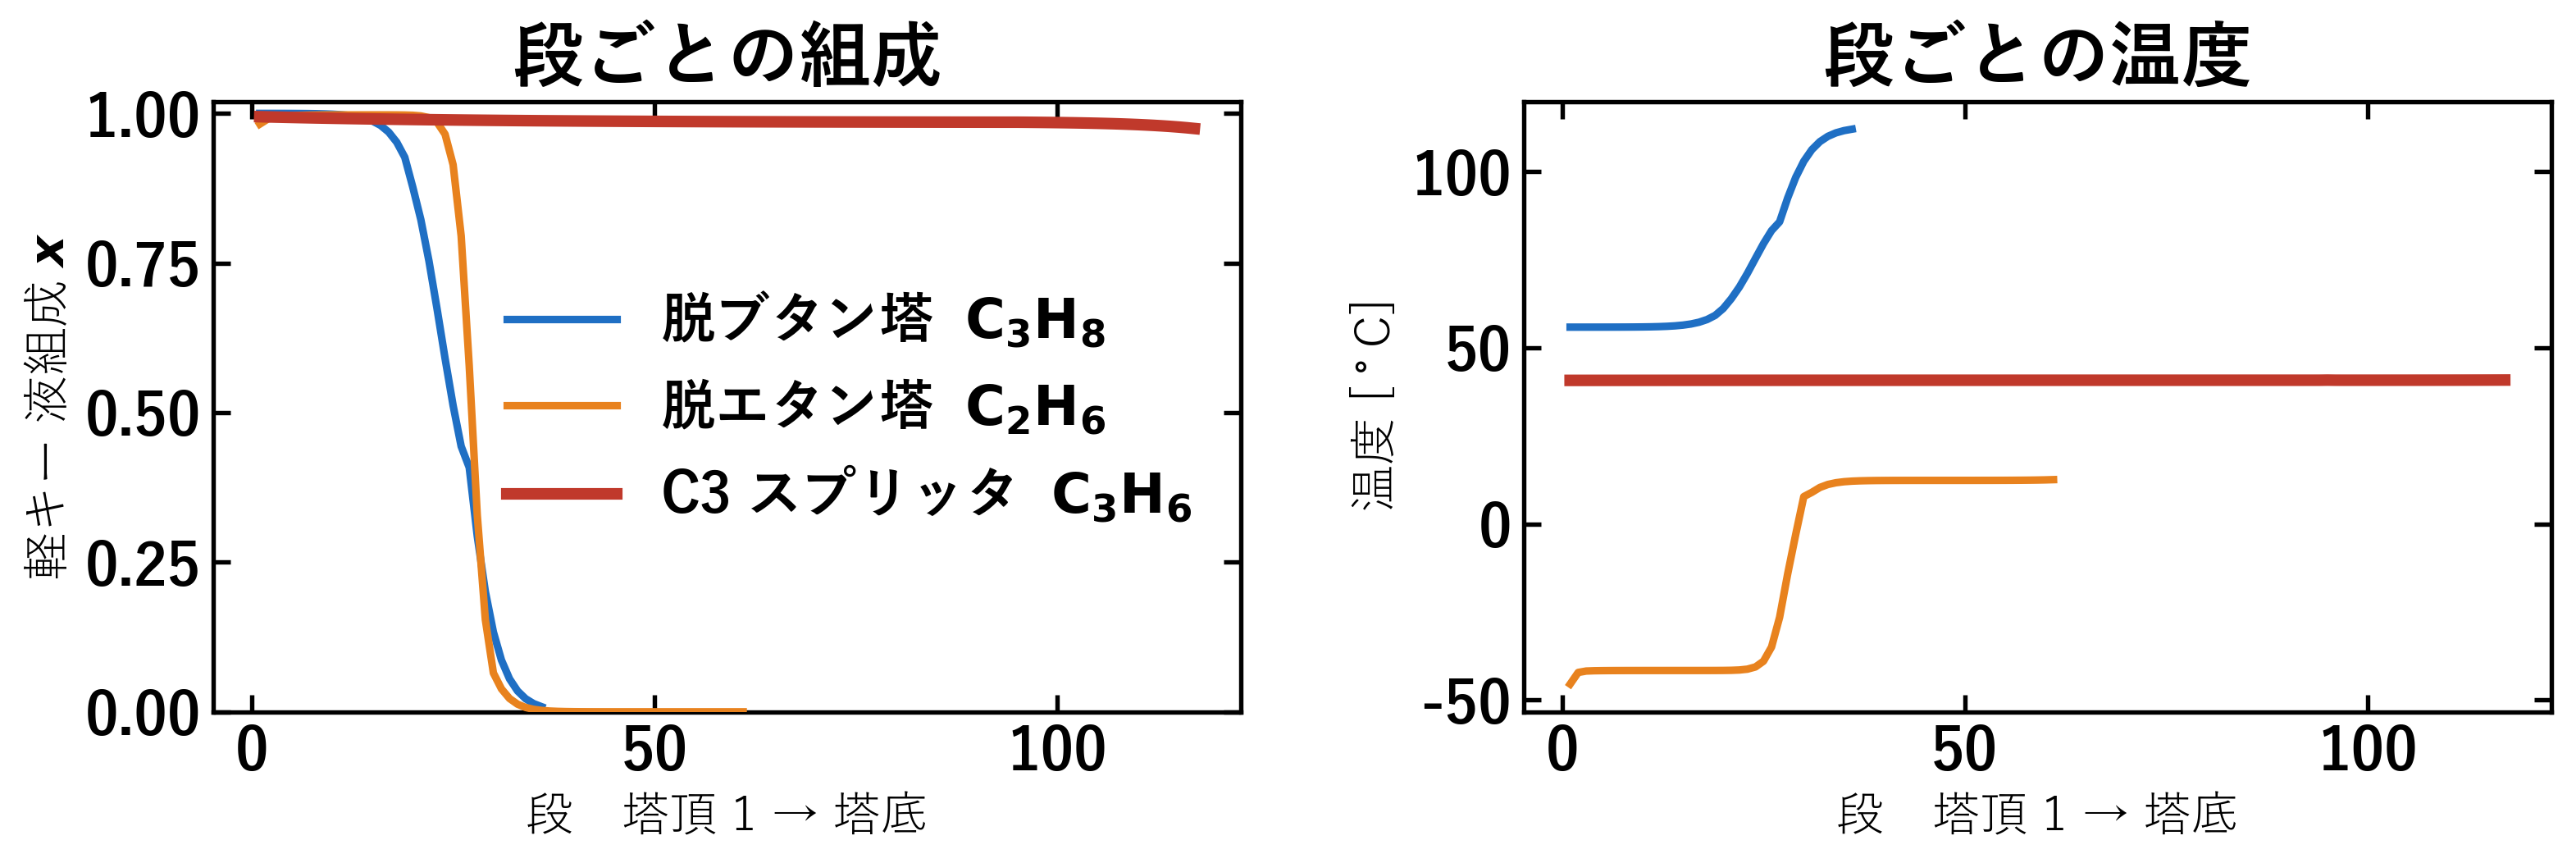
\includegraphics[width=0.97\linewidth]{dist_profiles}\par
  \vspace{0.12em}
  {\footnotesize\raggedright
   {\color{ArrowBlue}\textbf{脱ブタン}}・{\color{DipeOrange}\textbf{脱エタン}}：少ない段で組成・温度が急変化 ＝ 沸点差が大きく分離容易\par
   {\color{SpRed}\textbf{C3 スプリッタ}}：$117$ 段でも組成・温度ほぼ一定 ＝ 沸点差 $6$ K・$\alpha\!\approx\!1.07$ で分離困難\par}

\end{frame}

\end{document}
